\documentclass[12pt letterpaper]{article}

\usepackage{fullpage}
\usepackage{graphicx}
\usepackage{amsmath}

\providecommand{\e}[1]{\ensuremath{\times 10^{#1}}}
\usepackage{gensymb}

\usepackage{float}


\title{Math 448 -- Assignment \#8}
\author{Johnny Minor}
\date{\today}

\begin{document}
\maketitle

\noindent 2. a. 
\begin{verbatim}
max_error = 0.0132 
\end{verbatim}
\begin{figure}[H]
  \caption{Euler method and the true solution. }
  \centering
    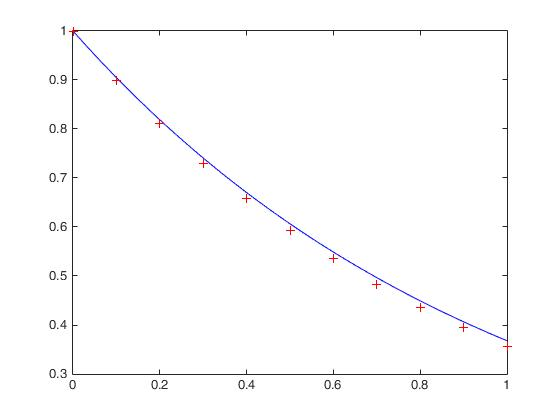
\includegraphics[width=.5\textwidth]{euler.jpg}
    \label{fig:Euler_2a}
\end{figure}

\noindent b. 
\begin{verbatim}
max_error = 0.0012 
\end{verbatim}
\begin{figure}[H]
  \caption{Heun method and the true solution.}
  \centering
    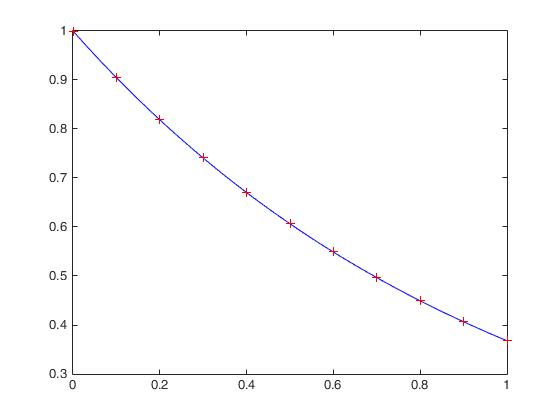
\includegraphics[width=.5\textwidth]{heuns.jpg}
    \label{fig:heun_2a}
\end{figure}

\noindent c. 
\begin{verbatim}
max_error = 0.0119 
\end{verbatim}
\begin{figure}[H]
  \caption{Backward Euler method and the true solution.}
  \centering
    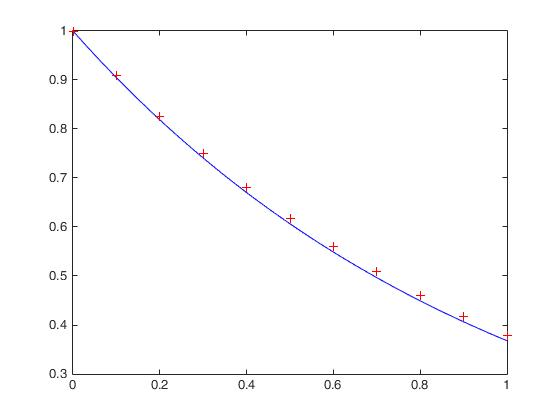
\includegraphics[width=.5\textwidth]{backward_euler.jpg}
    \label{fig:backward_2a}
\end{figure}

\noindent d. 
\begin{verbatim}
max_error = 2.0890e-04
\end{verbatim}
\begin{figure}[H]
  \caption{Trapezoid method and the true solution.}
  \centering
    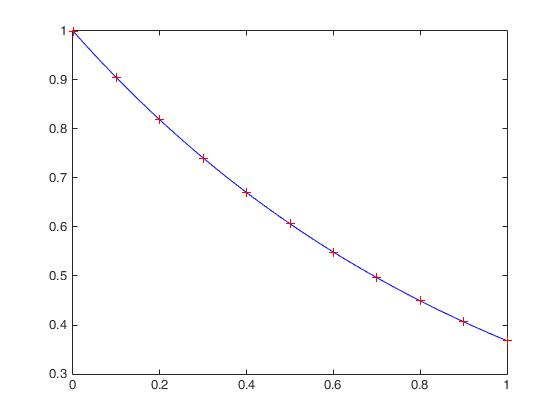
\includegraphics[width=.5\textwidth]{trapezoid.jpg}
    \label{fig:trapz}
\end{figure}

We can see that both first-order methods (Euler and backward Euler) are less accurate than the second-order methods 
(Heun and trapezoid). We can also see that the the implicit methods of the same order are better than the explicit methods. Meaning, that backward Euler is slightly more accurate than Euler, and trapezoidal is better than Heun. 


\noindent 3. a.
We would expect both Euler and Heun to do very poorly since they are not stiffly stable, and this is confirmed in this problem.  
\begin{verbatim}
max_error =  1.7029e+06
\end{verbatim}
\begin{figure}[H]
  \caption{Euler method and the true solution. }
  \centering
    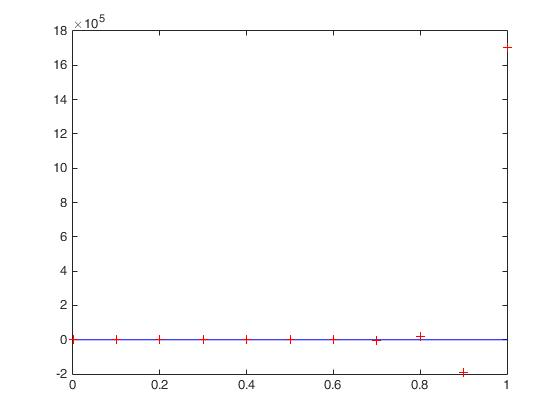
\includegraphics[width=.5\textwidth]{euler_stiff.jpg}
    \label{fig:Euler_3a}
\end{figure}

\noindent b. 
\begin{verbatim}
max_error = 8.0706e+12
\end{verbatim}
\begin{figure}[H]
  \caption{Heun method and the true solution.}
  \centering
    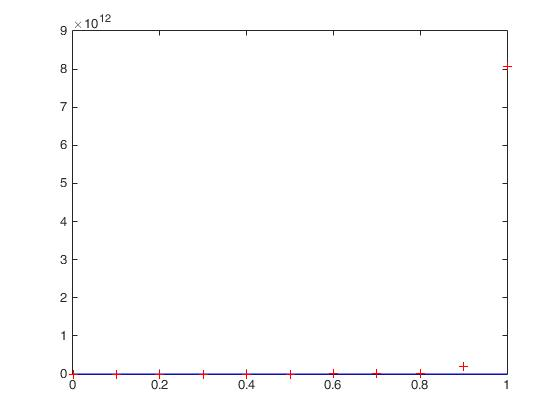
\includegraphics[width=.5\textwidth]{heuns_stiff.jpg}
    \label{fig:heun_3b}
\end{figure}

\noindent c. 
\begin{verbatim}
max_error = 4.2535e-04
\end{verbatim}
\begin{figure}[H]
  \caption{Backward Euler method and the true solution.}
  \centering
    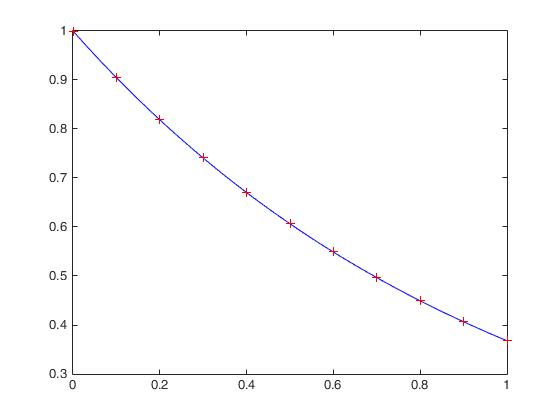
\includegraphics[width=.5\textwidth]{backward_euler_stiff.jpg}
    \label{fig:backward_3c}
\end{figure}

\noindent d. 
\begin{verbatim}
max_error = 1.3215e-05
\end{verbatim}
\begin{figure}[H]
  \caption{Trapezoid method and the true solution.}
  \centering
    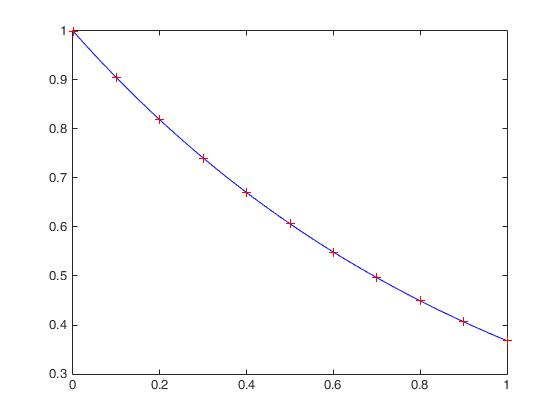
\includegraphics[width=.5\textwidth]{trapezoid_stiff.jpg}
    \label{fig:trapz}
\end{figure}

\noindent 4. 
It can be found that if we decrease h to 1/60 then we can finally get an accurate result using Euler and Heun. 
\begin{verbatim}
max_error =  1.3812e-04
\end{verbatim}
\begin{figure}[H]
  \caption{Euler method and the true solution. }
  \centering
    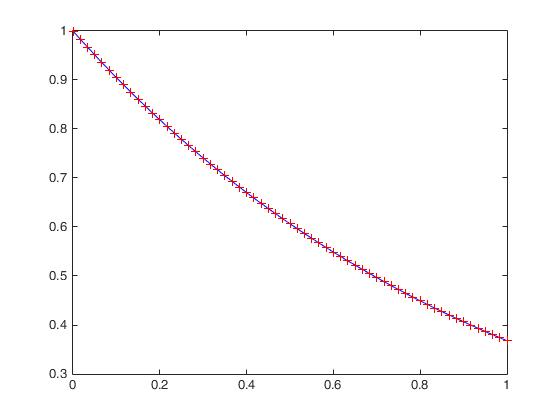
\includegraphics[width=.5\textwidth]{euler_stiff_smaller.jpg}
    \label{fig:Euler_4a}
\end{figure}

\noindent b. 
\begin{verbatim}
max_error = 3.5475e-04
\end{verbatim}
\begin{figure}[H]
  \caption{Heun method and the true solution.}
  \centering
    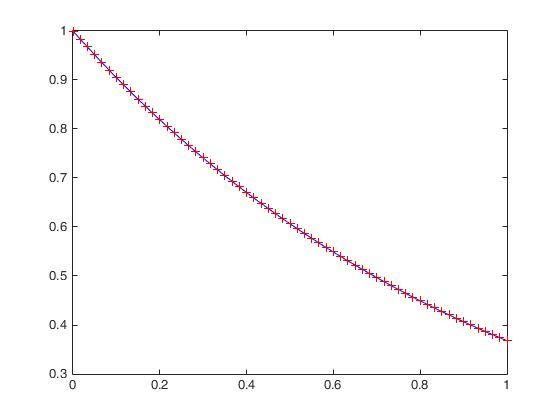
\includegraphics[width=.5\textwidth]{heuns_stiff_smaller.jpg}
    \label{fig:heun_4b}
\end{figure}

\noindent We can also try larger step sizes such as $h = 0.5$ and $h = 1.0$, and see that even with a larger step size we still get an accurate solution. 
\noindent c. 

\begin{verbatim}
max_error = 0.0010
\end{verbatim}
\begin{figure}[H]
  \caption{Trapezoid method with h=1.0 and the true solution.}
  \centering
    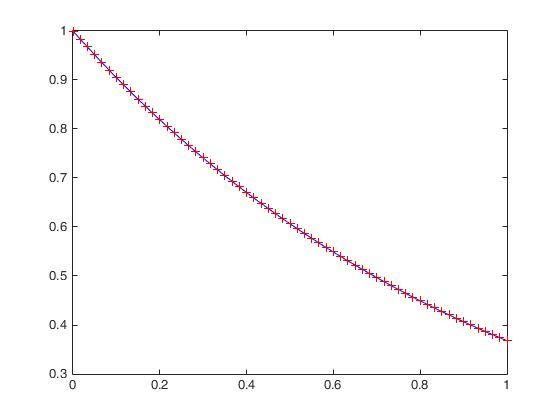
\includegraphics[width=.5\textwidth]{heuns_stiff_smaller.jpg}
    \label{fig:trapezoid_4}
\end{figure}



\end{document}